% Figure: Existing DMOSpeech 2 baseline handover architecture (Li et al., 2025 / infer.py)
\begin{figure}[!htbp]
\centering
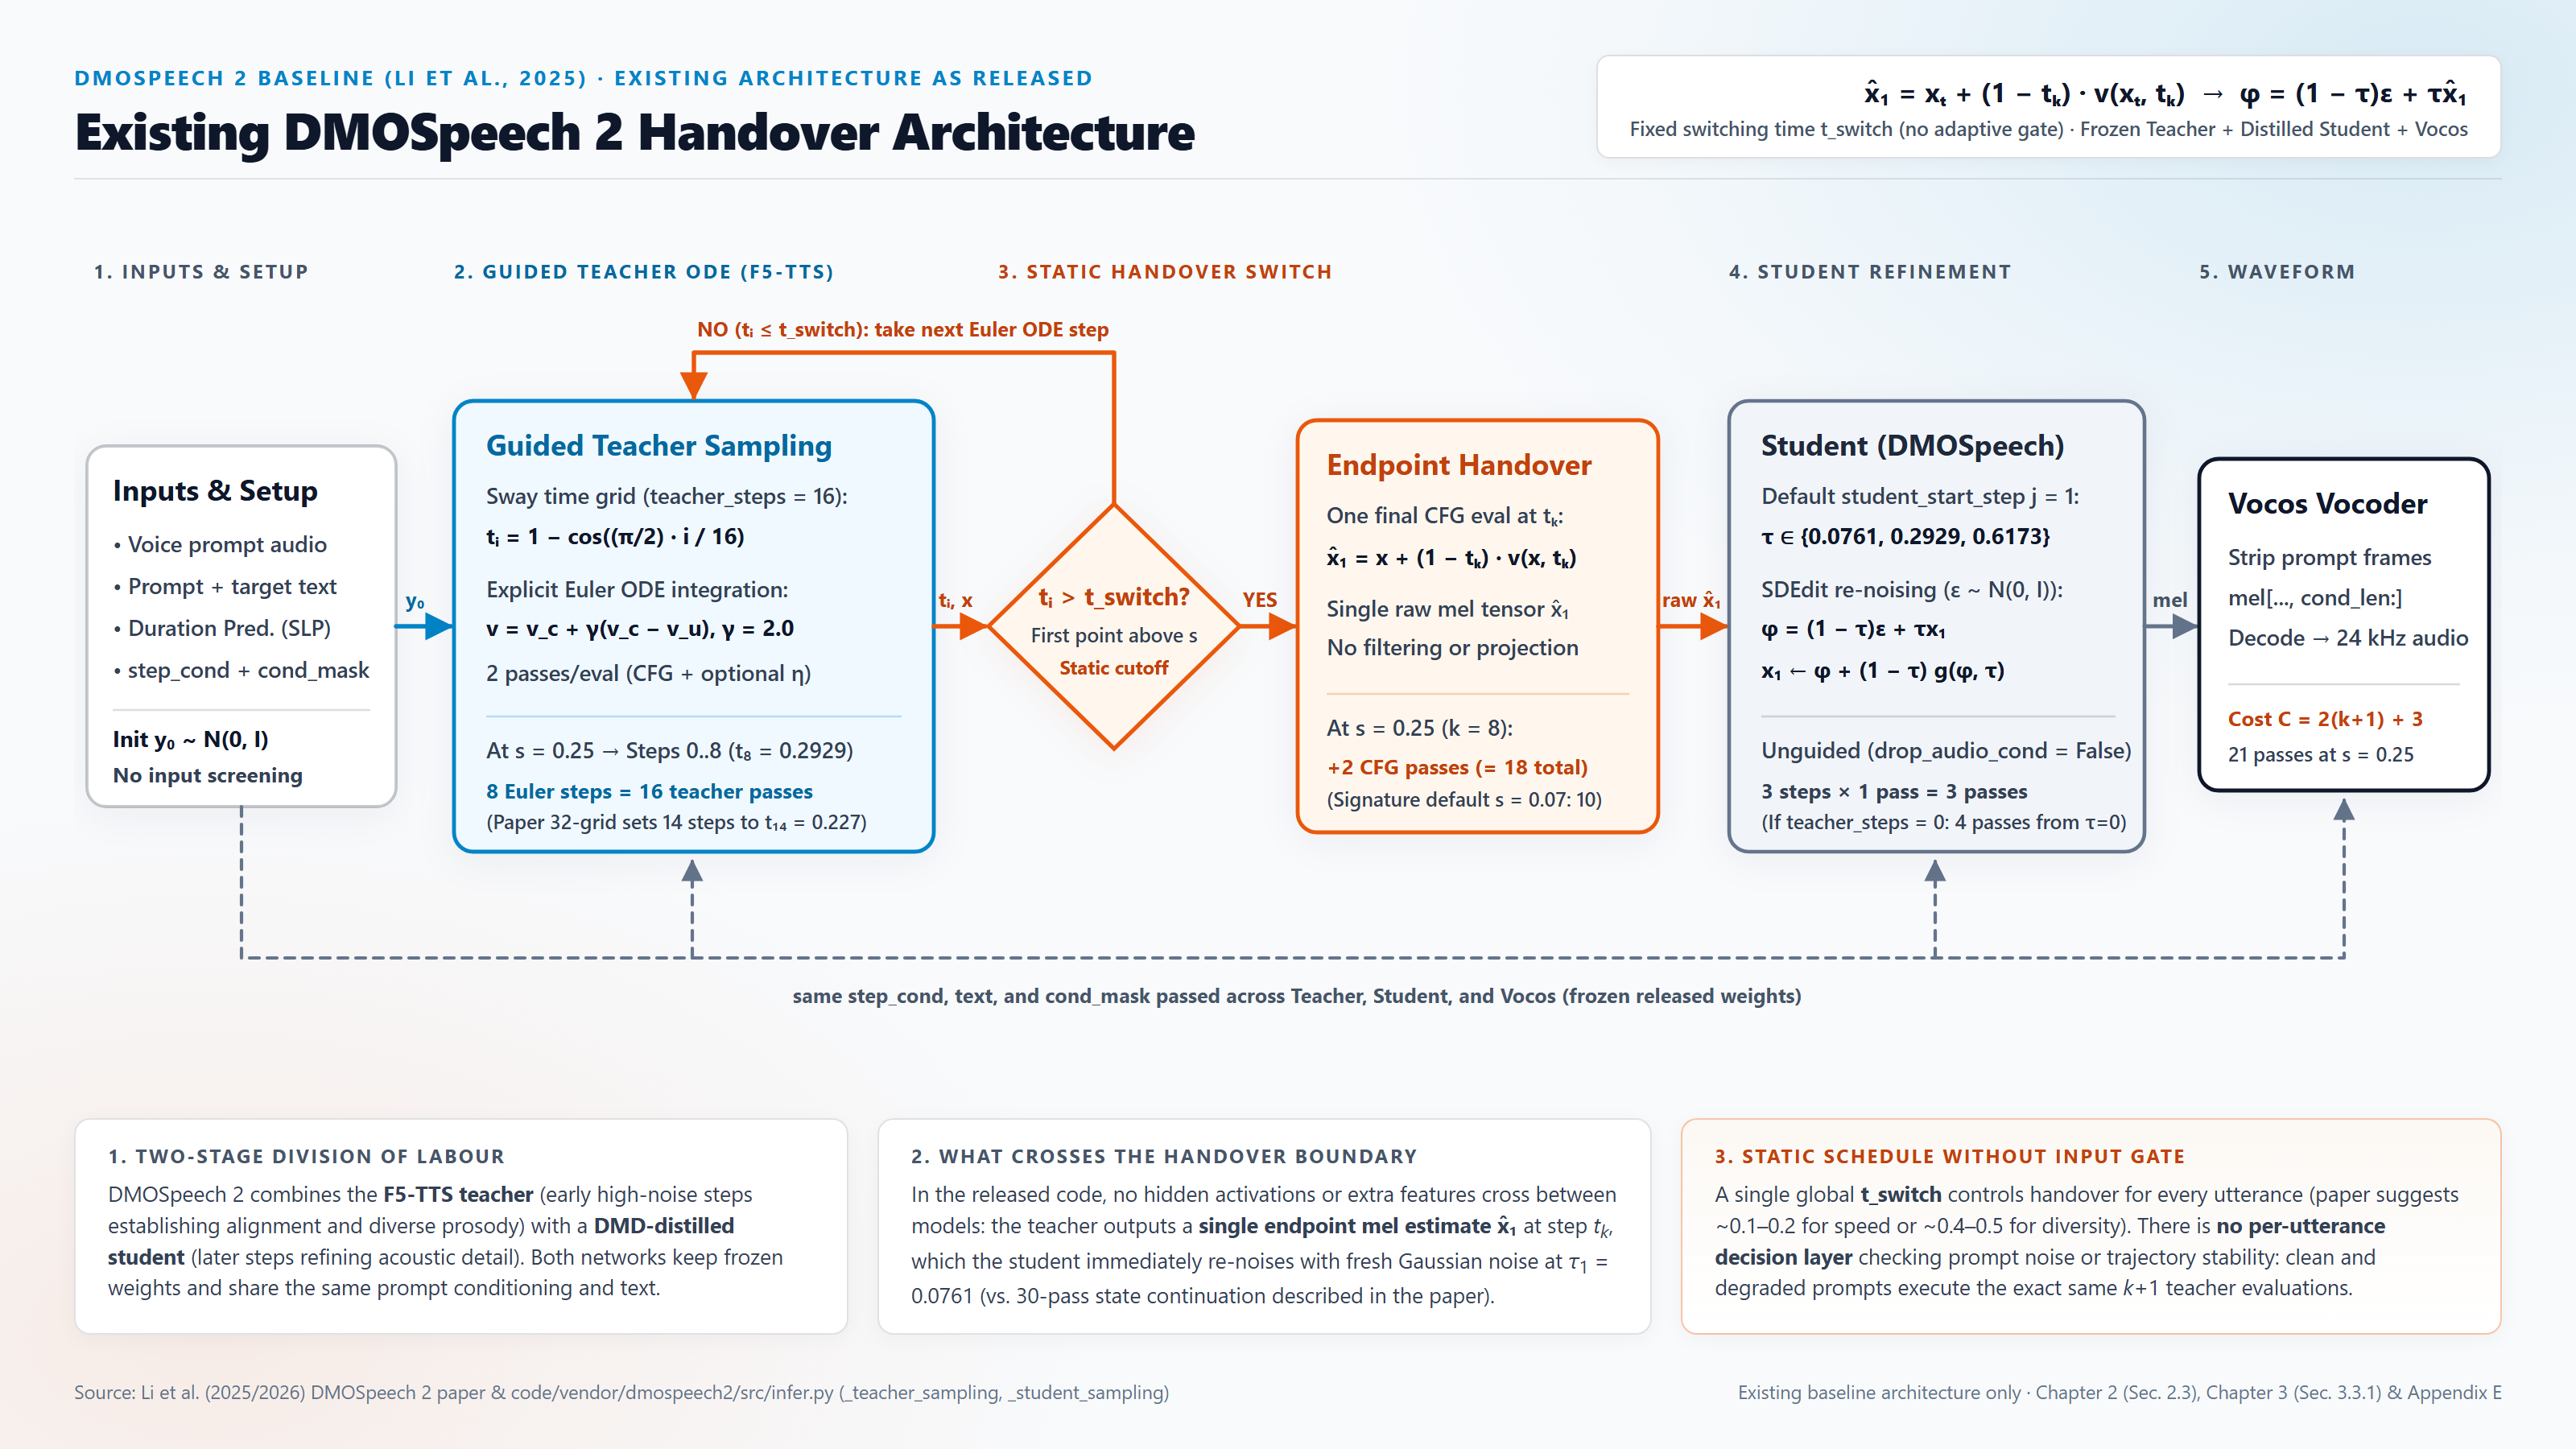
\includegraphics[width=\linewidth]{figures/baseline_handover_architectures.png}
\caption[Existing DMOSpeech~2 teacher-guided handover architecture (released baseline)]{Architecture of the existing DMOSpeech~2 baseline handover sampler \parencite{li2025dmospeech2,li2025dmospeech2code} without any added decision gate or payload router. In \nolinkurl{code/vendor/dmospeech2/src/infer.py}, guided \texttt{F5-TTS} integrates explicit Euler steps on a $16$-interval sway grid until the static cutoff $t_k > t_{\text{switch}}$ triggers one final conditional/unconditional evaluation for the raw endpoint mel tensor $\hat x_1$, which the \texttt{DMOSpeech} student re-noises at $j=1$ ($\tau_1=0.0761$) across three unguided refinement steps before \texttt{Vocos} decoding ($C = 2(k+1)+3 = 21$ passes at $s=0.25$, vs.\ $30$ passes in the paper's $32$-grid $14+2$ setup).}
\label{fig:baseline-handover}
\end{figure}
